\section{Goals}

In this paper, I examine the interfaces used to communicate music, and synthesise a working model of ways to notate techniques that can interface with traditional Western musical notation, and extend it.
The argument being put forth is that much like a language, music notation evolves naturally, with new `words' being developed when no suitable existing `word' is found.
The system which I propose is not a constructed language like Lojban or Esperanto, which take an opinionated and prescriptive approach to language. 
Rather, the method is more like compiling a list of morphemes, breaking down our existing language into its elements so that compoundment, affixation, and other methods of constructing new `words' may occur naturally.
With this system, we will be able to establish a dictionary of existing symbols, as well as their function.
Composers that seek to notate in new and different manners will be able to take the symbols and interfaces developed a la carte, and construct their own, specific to their needs; if a composer develops a work in which the state of the score changes, traditional notation may require a 

\section{Literature Review}
Of particular interest is the work of Ellen Fallowfield, whose thesis, `CelloMap' website and recently, application, form a comprehensive and holistic review of the ways in which a performer may `map' actions onto a cello.\autocite[]{fallowfieldCelloMapHandbook2009,fallowfieldCelloMap}
This non-opinionated and genericized method of cataloguing actions sees its contents applicable where a more specific approach would fall short, ensuring that it does not fall out of date.
In a similar way, I aim to catalogue and genericize actions from a composer's perspective, providing a suite of tools with which a composer can construct a notation to suit any \hl{FINISH SENTENCE}

\subsection{Argument}
In the 20th century, the `cult of the written score' developed, in which the composer prescribed more and more parameters to be interpreted literally.\autocite[]{citation very much needed}
This was in part fueled by contemporary composers being strongly opinionated in how their works should be interpreted, and partly because of the styles-- the sheer breadth of the number of parameters specified in New Complexicist works makes the interpreter pre-biased to assume that there is little room for interpretation.
This has permeated through to an underlying culture of assuming that when performing a work by a living composer that, if they wished for it to be interpreted a specific way, they would have specified that.
This obviation of interpreting the connotative in favour of the denotative 

Unfortunately, notation is an imperfect representation of the perfect, Platonic ideal, which exists only in the mind of the composer. 

As an example, John Fiske categorises \begin{quotation}
    denotation [as] what is photographed, connotation [as] how it is photographed
\end{quotation}.



This thesis aims to provide the composer with more tools to aid in the specificity of the work, so that they may more accurately and concisely communicate the desired techniques.
Approaching it from a 

\subsection{Semiotics}
A brief overview of semiotics is necessary in order for any serious discussion to be had.
Semiotics, the study of signs (read: meaningful communication), was invented concurrently by Ferdinand de Saussure and Charles Sanders Peirce independent of one another.
The most appreciable difference between their models was that while Saussure held that signs were made up of a signifier (the form of the sign) and signified (its meaning), Pierce's model also had an interpretant; the object that the audience interprets the signified as (since it is impossible to replicate meaning perfectly).
Signifiers are then broken up into three discrete categories; 
\begin{itemize}
\item \emph{\gls{icon}}: which have a direct physical connection to the signified. Photographs are an example of icons.
\item \emph{\gls{index}}: which show evidence of the signified. The most common example being smoke indexing fire.
\item \emph{\gls{symbol}}: which have no resemblance between the signifier and the signified; their meaning must be culturally learned. Arabic numerals, the radioactive symbol, and flags are all symbols.
\end{itemize}

Finally, our signs have two channels of information.
\begin{itemize}
\item \emph{\gls{denotation}}: the basic or literal meaning of the sign (i.e.\ a picture of a rose signifies the flower of the genus \emph{Rosa} of the family \emph{Rosaceae})
\item \emph{\gls{connotation}}: the secondary, culturally inferred meaning; a rose might also signify passion or love, depending on the context.
\end{itemize}

Interpreting these signs is described as semiosis, which Tagg states is `simply the process by which meaning is produced and understood.'\autocite[156]{taggMusicMeaningsModern2013}
Semiosis happens constantly; the process of converting these words into the understanding of the concept of semiosis is, in itself, semiosis. 
Pierce argues that in between the audience and the signifier, during the process of semiosis there is the interpretant, an object that the audience creates that represents the signified (because a dog cannot exist inside our heads, but merely the idea of a dog; the reality of the dog will never be fully realised inside the mind because it lacks the gestalt of the physical thing; 
it's a construct, unable to approach the truth of the dog by virtue of its limitations).
Semiosis is an important step, as the interpretant which Peirce describes is unique to the audience; we construct meaning completely independently, informed by our past experiences and knowledge.\citetemp{citation needed Pierce}
Thus, the same picture of an aunt's dog may be interpreted by the aunt as being a loving pet, whereas a neighbour might interpret the image more negatively, as `the annoying dog that wakes me up at 6am'.

Notation is the physical manifestation of a perfect ideal, imperfectly represented as best possible by the composer.


Floris Schuiling describes music notations as \begin{quotation}
`interfaces for imagining virtual musical relations'
\end{quotation}
which is an \hl{FINISH SENTENCE}
Looking at Western notation, we have several instances where a symbol may hold a different context depending on the interpreter's experience-- 
the same notation is used for a harmonic and a note that is meant to be played open on a French horn.\autocite[]{schuilingNotationCulturesEthnomusicology2019}
If a musician was given a piece of sheet music without any indicator of the instrument that it was written for, their experience (or lack thereof) with one of the instruments may influence how they choose to interpret the symbol.

Semiotics has seen a resurgence of interest with web design, where intuitive `notation' is sought after to reduce the `friction', or difficulty a user has navigating a site.
We can learn many things from the research that has been done into how to use skeuomorphic design to convey an element's function.
Our goal with constructing intuitive music notation is to reduce the `friction' just like a web designer.
We can use the connotations of existing symbols to help infer how we can construct new symbols.
As an example, the line that makes up a glissandi can be either straight, or wavy, as seen in \autoref{fig:Glissando}.
\begin{figure}
    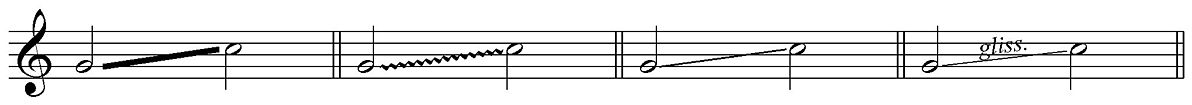
\includegraphics[]{./resources/glissando.jpg}
\caption{Various styles of glissandi}\label{fig:Glissando}
\end{figure}
The similarity of the last two examples on the right to the notation for \emph{portamento} results in a connotation with those two types being continuous, rather than having discrete pitches.
Additionally, the interpretant's instrument may also influence the meaning to them- timpanists and trombonists are more likely to interpret glissandi as continuous changes, while pianists interpret step-wise due to the nature of their instruments.\autocite[]{}

Lastly, we need to understand that some symbols are not compatible with one another; a properly engraved work will never have an upbow and downbow on the same note, as the two symbols fulfill the same function.
This is what is known as a paradigmatic relationship; by virtue of the presence of one, it excludes the possibility of the other.
Other examples of paradigms would be the degree at which a French horn opens or mutes their instrument.
Looking at web design, we can draw a somewhat rough parallel to drop-down menus; there's only one slot that can be filled.

\hl{FINISH ARGUMENT}